\begin{surferPage}{Eine $A_4^{+-}$ Singularität}
 Eine $A_4^{+-}$ Singularität mit Gleichung sieht im
    Wesentlichen gleich 
    aus wie jede andere $A_{2k}^{+-}$, $k\ge 1$ Singularität, wie man schon
    von der Gleichung
    \[x^{2k+1}+y^2-z^2=0\]
    erahnen kann.
    Der einzige Unterschied zur $A_2^{+-}$ Singularität (linkes Bild, in der
    Mitte $A_4^{+-}$, rechts $A_6^{+-}$) ist Berühr-Ordnung:
    \vspace*{-0.5em}
    \begin{center}
      \begin{tabular}{c@{\quad}c@{\quad}c}
        \begin{tabular}{@{}c@{}}
          
\includegraphics[width=1.2cm]{../../common/images/A2pm}
        \end{tabular}
        &
        \begin{tabular}{@{}c@{}}
          
\includegraphics[width=1.2cm]{../../common/images/A4pm}
        \end{tabular}
        &
        \begin{tabular}{@{}c@{}}
          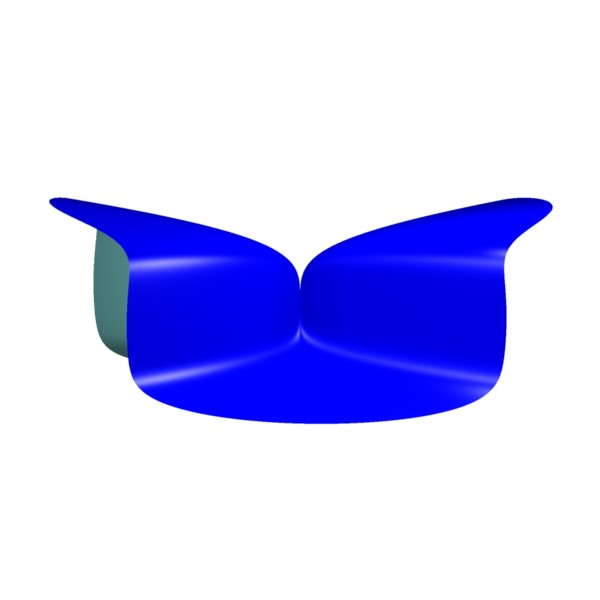
\includegraphics[width=1.2cm]{../../common/images/A6pm}
        \end{tabular}
      \end{tabular}
    \end{center}
    \vspace*{-0.4em}
    Einen wesentlich größeren Unterschied erkennt man, wenn man versucht,
    diese Singularitäten entweder in eine Fläche mit möglichst vielen
    Doppelkegeln oder in eine Fläche mit möglichst vielen Durchgängen zu
    deformieren.
    Für eine $A_4^{+-}$ Singularität kann man nämlich $4$  (zwei von
    jeder Seite im Bild unten) statt der für
    die $A_2^{+-}$ Singularität möglichen $2$ Durchgänge produzieren:
    \begin{center}
      \vspace{-0.1cm}
      \begin{tabular}{@{}c@{\quad}c@{}}
        \begin{tabular}{@{}c@{}}
          
\includegraphics[width=1.2cm]{../../common/images/A4pm_sm_0}
        \end{tabular}
        &
        \begin{tabular}{@{}c@{}}
          
\includegraphics[width=1.2cm]{../../common/images/A4pm_sm_1}
        \end{tabular}
      \end{tabular}
    \end{center}
%     \dontshow{
%     % 
%     \begin{center}
%       \vspace{-0.1cm}
%       \begin{tabular}{@{}c@{\quad}c@{\quad}c@{}}
%         \begin{tabular}{@{}c@{}}
%           
\includegraphics[width=1.2cm]{../../common/images/A4pm_0}
%         \end{tabular}
%         &
%         \begin{tabular}{@{}c@{}}
%           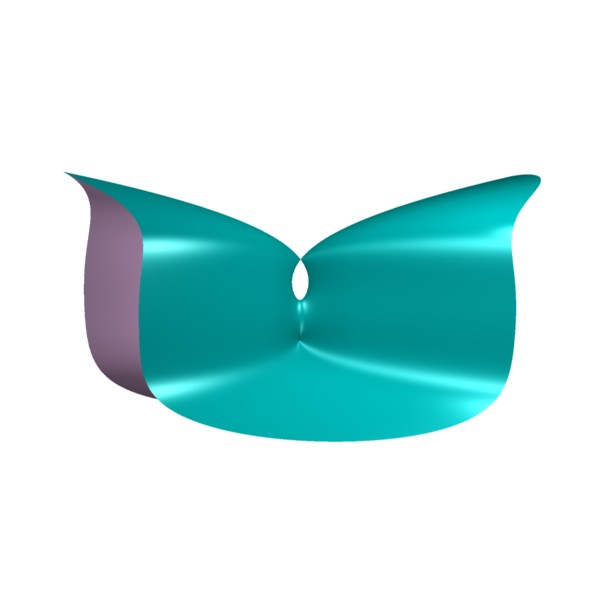
\includegraphics[width=1.2cm]{../../common/images/A4pm_1}
%         \end{tabular}
%         &
%         \begin{tabular}{@{}c@{}}
%           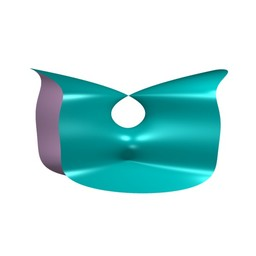
\includegraphics[width=1.2cm]{../../common/images/A4pm_2}
%         \end{tabular}
%       \end{tabular}
%     \end{center}
%     }
 
\end{surferPage}
